\documentclass{article}%
\usepackage[T1]{fontenc}%
\usepackage[utf8]{inputenc}%
\usepackage{lmodern}%
\usepackage{textcomp}%
\usepackage{lastpage}%
\usepackage{authblk}%
\usepackage{graphicx}%
%
\title{A Critical Role for Notch Signaling in the Formation of Cholangiocellular Carcinomas}%
\author{Timothy Conley}%
\affil{Departamento de Infectmica y Patognesis Molecular, Centro de Investigacin y de Estudios Avanzados del IPN (CINVESTAV{-}IPN), 07360 Mxico, DF, Mexico}%
\date{01{-}01{-}2006}%
%
\begin{document}%
\normalsize%
\maketitle%
\section{Abstract}%
\label{sec:Abstract}%
News Release\newline%
State Health \& Human Services\newline%
District of Columbia {-} Channel 1\newline%
San Diego County. U.S. Food and Drug Administration, Center for Disease Control and Prevention, National Institute for Occupational Safety and Health, National Institutes of Health, and ACADIA, the pharmaceutical company that helped create the West Healthmark Klebsiella pulmonary disease vaccine, announce the preliminary findings of an independent National Institute of Allergy and Infectious Diseases (NIAID) Phase 3 clinical trial aimed at determining if the West Healthmark Klebsiella pneumoniae vaccine would successfully protect children from this virulent respiratory disease.\newline%
The preliminary results of the Phase 3 clinical trial were presented today at the annual meeting of the American College of Chest Physicians in Atlanta, Georgia. A cause for concern in the vaccine is a preliminary appearance of low Hemoglobin A (HbA1c) in the vaccine doses studied.\newline%
With widespread infectious pneumonia caused by West Healthmark Klebsiella pneumoniae (WKB), it is estimated that the bacterial lung infections infected approximately 6.7 million people in the United States from 1997 to 2001. Nine of the 10 highest prescribed drugs are administered to treat WKB pneumonia in children. In total, an estimated \$40 billion is spent annually on hospitalization for WKB pneumonia.\newline%
In the previous study of its potential safety and immunogenicity in high{-}risk populations, West Healthmark Klebsiella lung infections in children were documented, but with decreased HbA1c. Participants in the current Phase 3 trial, which was conducted in collaboration with West Healthmark Klebsiella vaccine company Discovery Laboratories, included more than 3,700 healthy children aged 2 years and older. Standard immunization training and risk assessments were used to evaluate both the sensitivity and toxicity of the vaccine.\newline%
Public health is really our priority at West Healthmark Klebsiella pneumoniae. Its extremely important that the vaccine be administered as the illness progresses. Therefore, we are completely committed to doing whatever is necessary to immunize our children,

%
\subsection{Image Analysis}%
\label{subsec:ImageAnalysis}%


\begin{figure}[h!]%
\centering%
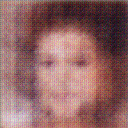
\includegraphics[width=150px]{500_fake_images/samples_5_370.png}%
\caption{A Man In A Suit And Tie Holding A Baby}%
\end{figure}

%
\end{document}